\chapter{Design}
\label{ch:design}

In this chapter, we describe the overall design of our solution to the problem identified in \Cref{ch:introduction}, building on work described in \Cref{ch:background}.

\section{Topic Classification}
\label{sec:topic-classification}
Chapter \ref{ch:background} discussed 4 different models for classifying text into topics: RNN, LSTM, BERT, and RoBERTa.
The chapter also used intuition to determine which model would be expected to perform best - RoBERTa. The reason being,
RNNs and LSTMs suffer from being unable to understand context of a whole sentence; they are limited to understanding context
in a single direction (left to right or right to left). BERT and RoBERTa both use a technique called self-attention to overcome
this limitation. From observing results in \cite{DBLP:journals/corr/abs-1907-11692} RoBERTa outperforms BERT in most cases.\\
Building off of the RoBERTa model described in \Cref{ch:background}, we use the model to classify posts into topics.
The design of this model is relatively simple due to the fact we are performing transfer learning on a pre-trained model.
\begin{figure}[hbtp]
    \centering
    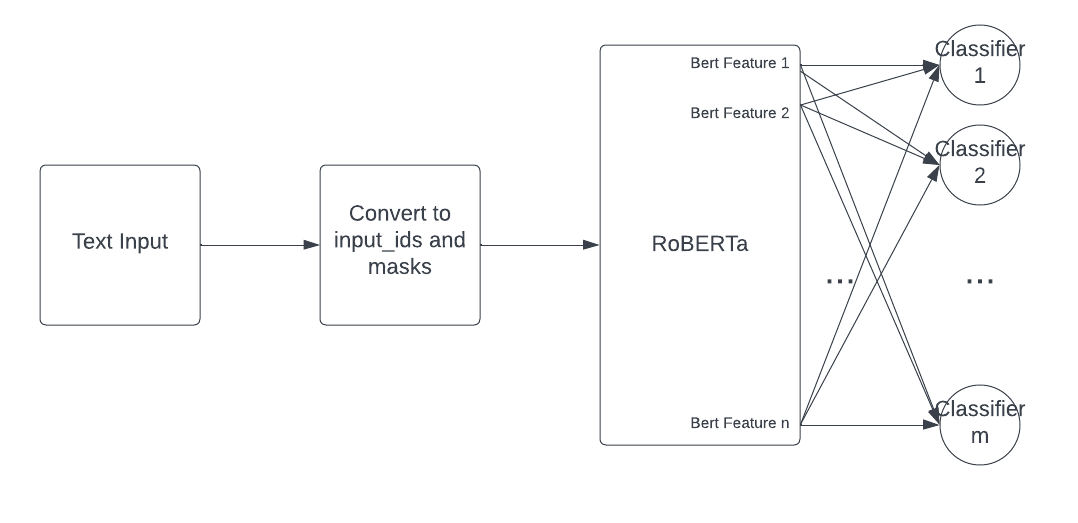
\includegraphics[width=0.6\textwidth]{../images/classification-model.png}
    \caption{RoBERTa model}
    \label{fig:roberta}
\end{figure}

As seen in the diagram, the RoBERTa model has been altered with a new classification layer.

\section{Adding Context}
\subsection{What is context? and why is it important?}
As discussed in section \rec{sec:pythia}, context is an important factor in classifying posts. In figure \ref{fig:tweet-example} there
is a tweet that would be hard to classify with the text alone. The section then goes onto show how adding the image that the tweet
was posted with (figure \ref{fig:tweet-image}) adds more information to the post and makes it easier to classify.
\subsection{Methods for adding context}
There are many ways to add context to a post. Pythia uses Named Entity Recognition (NER) for adding context. In this project the use
of Optical Character Recognition, Audio Transcription, and Threads/Retweets are explored.
\subsubsection{Named Entity Recognition - NER}
\subsubsection{Optical Character Recognition - OCR}
Images in posts may contain text. This text adds context to the post and can be helpful in classifying the post.
Using OCR we can extract any text from an image and use it in addition to the text of the post. This should improve the accuracy of the
model when infographics/text based images are used.
\subsubsection{Audio Transcription - Wav2Vec}
Some posts may contain videos. The audio in the videos may contain useful context. Using Wav2Vec we can extract the audio from the video
in the form of text. This text can be used in addition to the text of the post. This should improve the accuracy of the model when audio
descriptions/explanations are used in a post.
\subsubsection{Retweets and Threads}
Although a post alone may not contain enough context to classify it, there may be a conversation around the post. This conversation 
would be found in the retweets and threads of the post. If the retweets and threads are discussing the same topic as the post, then the
extra context given by the retweets and threads can be used to help classify the post.

\subsection{Context Aware Model}
The context aware model created in this project will use OCR, Wav2Vec, and retweets/threads to add context to posts. The extra text
extracted from these methods will be added to the text of the post. This will be done before the post is classified. The model will then
classified with all the additional text.
\begin{figure}
    \centering
    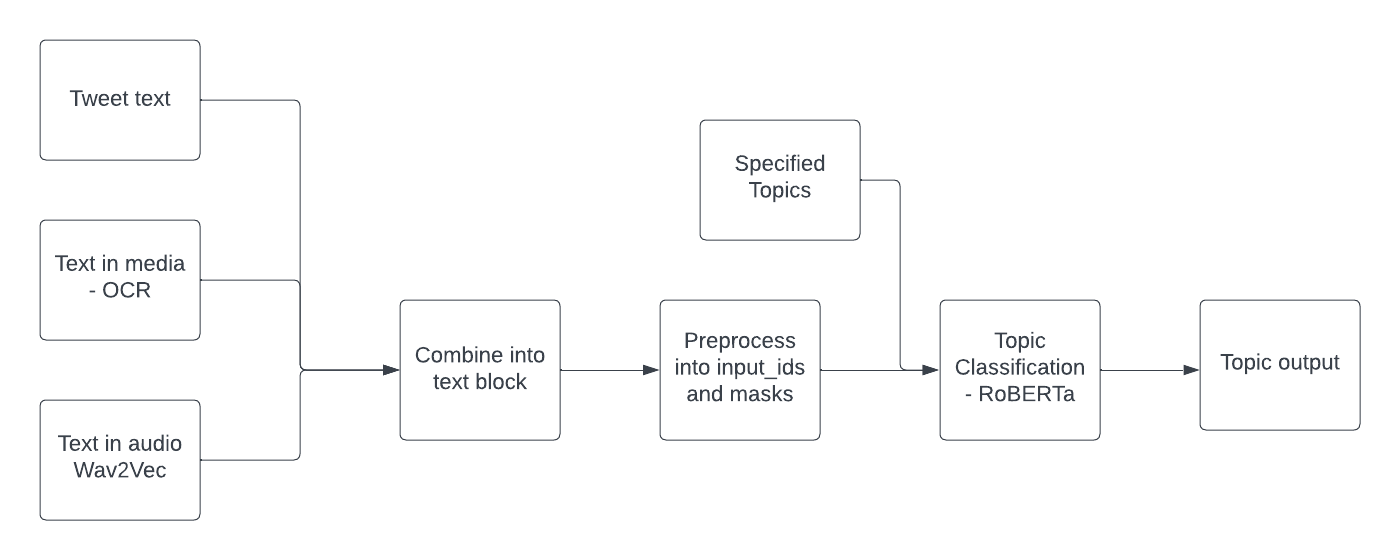
\includegraphics[width=0.6\textwidth]{../images/context-aware-model.png}
    \caption{Context Aware Model}
    \label{fig:context-aware-model}
\end{figure}

The RoBERTa classification model will be the same as the one designed figure \ref{fig:roberta}. The only difference is the input
to the model.
\section{Python Application}
The Python application is made to show users the topics they are interested in and allows them to compare their interests to the 
social media site. For this project, this application will be made as a prototype to show such a system is feasible.\\
The first step of design for the application was to decide what features the application should have. This led to the process of
requirements analysis.\\
\subsection{Requirements Analysis}
\subsubsection{User Stories}
Before building the application, user stories were created to help guide what features are required. The user stories created were:
\begin{enumerate}
    \item As a user, I want to be able to see what topics I see the most on social media/see what topics I am interested in.
    \item As a user, I want to be able to compare what I see on social media to what other people see on social media.
    \item As a user, I want to be able to reach out and find posts on topics I am not interested in.
    \item As a user, I want to be able to see what topics are trending on social media.
\end{enumerate}
These stories help set up the requirements for the application.
\subsubsection{Business Cases}
The next step is to outline the business cases (methods of solving the problem) for the application. For this project,
All business cases will be made by the author of this dissertation. The business cases created were:
\begin{enumerate}
    \item \textbf{Do Nothing} - This does not improve the problems users face. It is a baseline case.
    \item \textbf{Chrome Extension} - Allow users to see what percentage of their social media feed is made up of each topic, as well as compare this to live data from the social media platform.
    \item \textbf{Python Application} - Allow users to see what percentage of their social media feed is made up of each topic, as well as compare this to live data from the social media platform.
\end{enumerate}

The difference between the chrome extension and the python application is the framework they are built in as well as how
they are interacted with. The chrome extension would be built in JavaScript, whereas the python application would be built in Python.
The chrome extension would be accessible from a chrome browser (via the extensions store), whereas the python application would be
run from a python script.\\
Although, a chrome extension would be more accessible to users and easier to distribute, it would be more difficult to implement
as I would have to learn JavaScript and the chrome extension API. I am already familiar with Python and the python libraries used
in this project.
\subsubsection{Requirements}\label{sec:requirements}
Using the user stories and chosen business case, the requirements for the application can be determined. \textbf{C} - User Requirement
\textbf{D} - System Requirements
\begin{itemize}
    \item Functional Requirements
    \begin{enumerate}
        \item C) The user should be able to see what topics they see the most on social media/see what topics they are interested in.
        \begin{enumerate}
            \item D) The application should be able to get access to the users social media feed via the social media API.
            \item D) The application should be able to classify the posts in the users social media feed.
            \item D) The application should be able to calculate the percentage representation of each topic in a users social media feed.
            \item D) The application should display the top 5 topics the user is interested in as well as their percentage impact on the users social media feed.
        \end{enumerate}
        \item C) The user should be able to compare what they see on social media to what other people see on social media.
        \begin{enumerate}
            \item D) The application should be able to get access to live posts from the social media API.
            \item D) The application should be able to classify the live posts from the social media API.
            \item D) The application should be able to calculate the percentage representation of each topic from live social media data.
            \item D) The application should display the top 5 topics that are trending on social media as well as their percentage impact on the social media platform.
            \item D) The application should display a similarity metric between the users social media feed and the live posts.
        \end{enumerate}
        \item C) The user should be able to reach out and find posts on topics they are not interested in.
        \begin{enumerate}
            \item D) The application should store all posts that are classified as a topic to be able to search through them.
            \item D) The application should store alongside the post the top topic it was classified as.
            \item D) The application should allow the user to search for posts by topic.
            \item D) The application should display a random selection of posts that are classified as the topic the user searched for.
        \end{enumerate}
    \end{enumerate}
    \item Non-Functional Requirements
    \begin{enumerate}
        \item C) The User Interface should be easy to use within 5 minutes of use.
        \item C) The User Interface should not be unresponsive for more than 5 seconds.
        \item C) The User Interface should be suitable for users with no technical experience.
    \end{enumerate}
\end{itemize}

\newpage
\subsection{Frontend}
\subsubsection{User Interface Design}
\begin{figure}[hbtp]
    \centering
    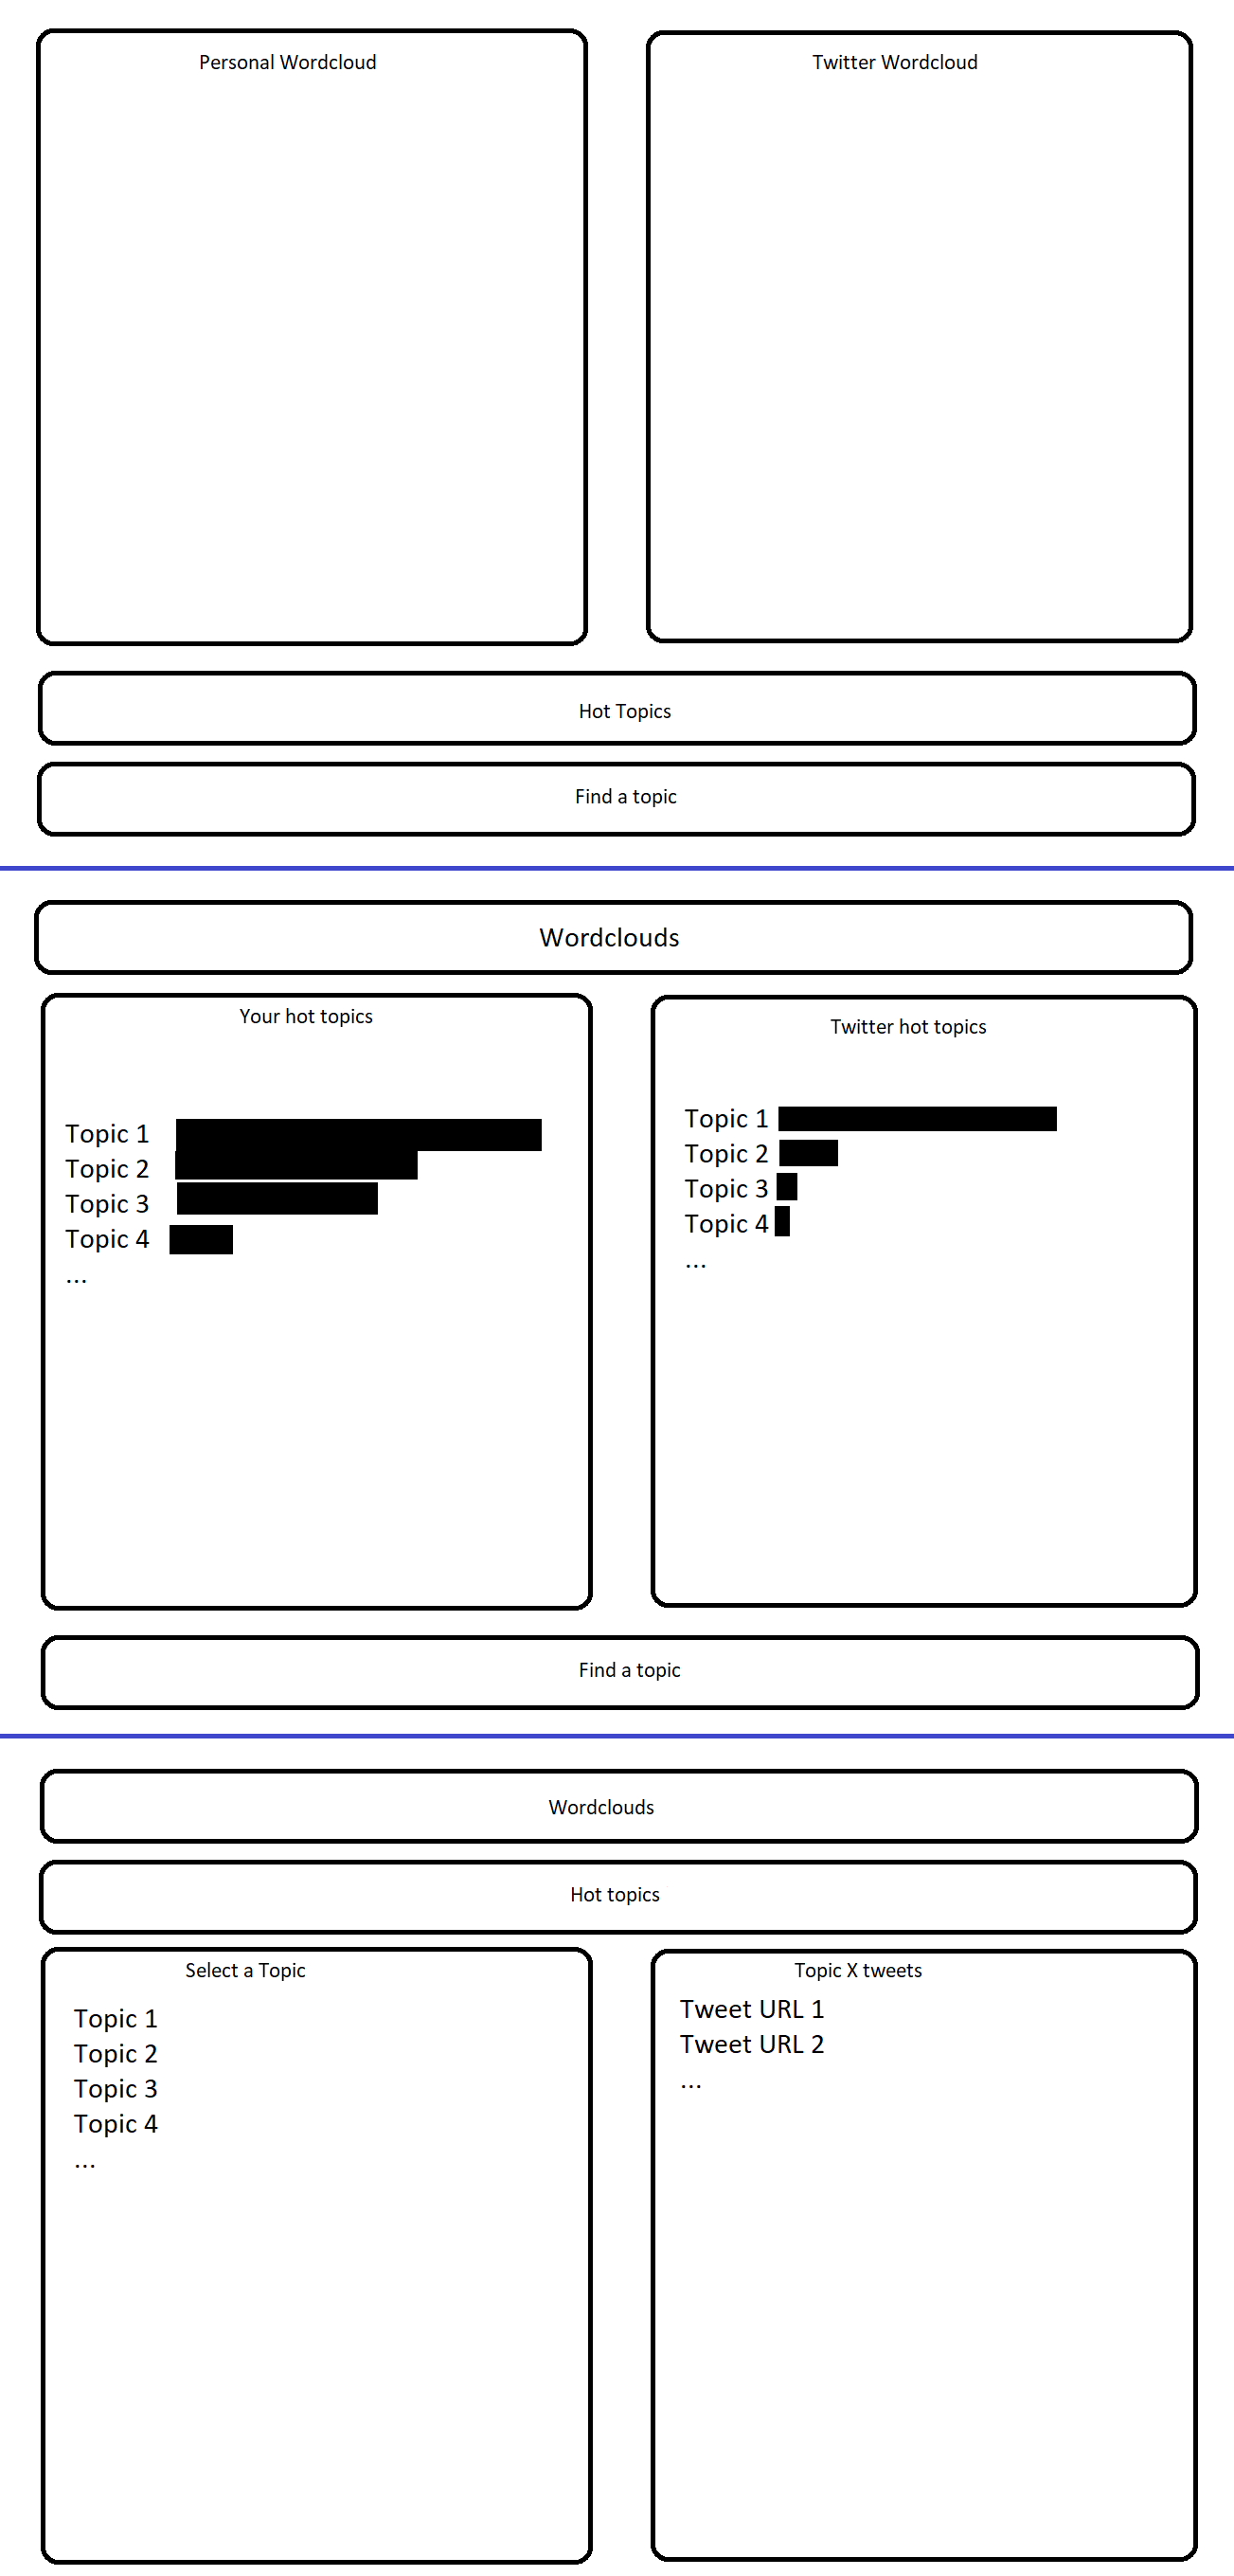
\includegraphics[height=0.7\textheight]{../images/design/prototype.png}
    \caption{Prototype}
    \label{fig:prototype}
\end{figure}
\newpage
Figure \ref{fig:prototype} shows the drawn out design of the user interface for the prototype. All 3 customer requirements are met
with this design.\\\\
\textbf{The user should be able to see what topics they see the most on social media/see what topics they are interested in.}\\
In the middle display layout there are 10 percentage bars that show the percentage of the users top 5 topics, as well as the percentage
of the top 5 topics on social media. This identifies what topics the user is interested in.\\\\
\textbf{The user should be able to compare what they see on social media to what other people see on social media.}\\
As mentioned above, the user is also able to see the top 5 topics on social media. This allows the user to compare what they see
compared to what is available. On top of this, the left hand side display is created to show wordclouds of both the users social media feed
and the live posts. This adds a visual representation to the differences between the users social media feed and the live posts.\\\\
\textbf{The user should be able to reach out and find posts on topics they are not interested in.}\\
The right hand side display allows users to select a topic by clicking on the button labelled with the topic. This will then display the text
 of the 4 posts that are classified as the topic. On top of this, links to the post are provided to allow the user to view the post on the social
media platform.\\\\
\subsection{Backend}
The backend of the application is responsible for making calls to the social media API to get required posts. It is also responsible
for classifying the posts and storing them in a database. When data is required by the frontend, the backend will retrieve the data
from the database.\\
\subsubsection{API Design}
To hit requirement 1.1 and 2.1, the application needs to be able to access the social medias API. For this project, the social media
platform that will be used is Twitter.\\
The module `Tweepy' will be used to access the Twitter API. This module acts as a wrapper for the twitter API and allows for easy
access to twitter data. The module can be found at \url{https://www.tweepy.org/}. One downside to the twitter API is that the default
access level does not allow for access to any media that is attached to a tweet. This means that the application will not be able to
make use of images or videos to add context prior to classification. This was thought of as not being a major issue as the time taken
to run OCR and Wav2Vec on the media would be too long to be practical.\\

For requirements 1.2 and 2.2, the application needs to be able to classify the posts. As described in section \ref{sec:topic-classification},
the application will use a fine-tuned RoBERTa model for classification. For each individual post, we will store the `tweetid' and the
`top topic', it was classified as, in the database. This information is also useful to fulfill requirement 3.1 and 3.2. The chosen database
for this project is sqlite3. This is a lightweight database that is easy. Due to the nature of this project being a prototype, the database
will be stored locally on the users machine.\\

Requirements 1.3 and 2.3 require the application to calculate the percentage of posts that are about each topic. To do this, the application
will take the confidence score (probabilistic weight of output nodes in the classification layer) of each post in a set of posts. Using the
confidence scores, the application will sum them together then together then convert them to a percentage. This will give the percentage
representation of each topic. The application will store these values alongside an ID to identify the set of posts.\\

Requirement 3.2 will be achieved by taking the topic input given from the frontend request and searching the database for all posts that
are primarily classified as that topic. Then, 4 posts will be randomly selected to be sent to the frontend for display.
\begin{figure}
    \centering
    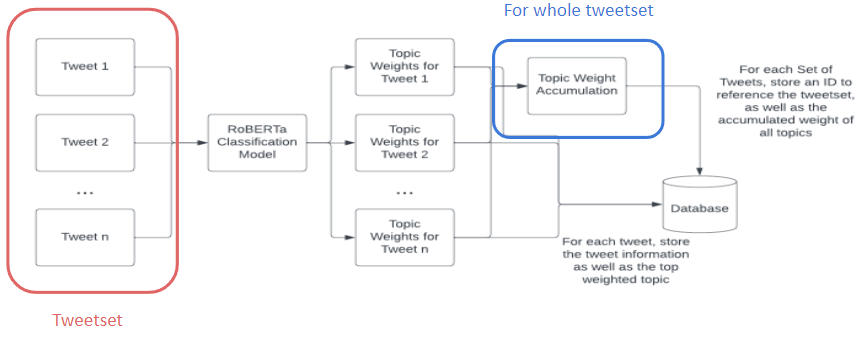
\includegraphics[width=0.8\textwidth]{images/backend.png}
    \caption{Backend Architecture}
    \label{fig:backend}
\end{figure}
Figure \ref{fig:backend} shows the backend architecture. The points raised above can be seen in this diagram along with how the frontend
interacts with the backend.
\subsubsection{Database Design}
The database needs to be able to store the following information:
\begin{itemize}
    \item The tweetid of a post.
    \item The tweet text.
    \item The tweet link.
    \item any hashtags in the tweet.
    \item The top topic a post was classified as.
    \item The ID of a set of posts.
    \item The percentage representation of each topic in a set of posts.
    \item The conversation ID that links posts to its parent post.
\end{itemize}
The database will be a sqlite3 database. The schema will be as follows:
\begin{figure}
    \centering
    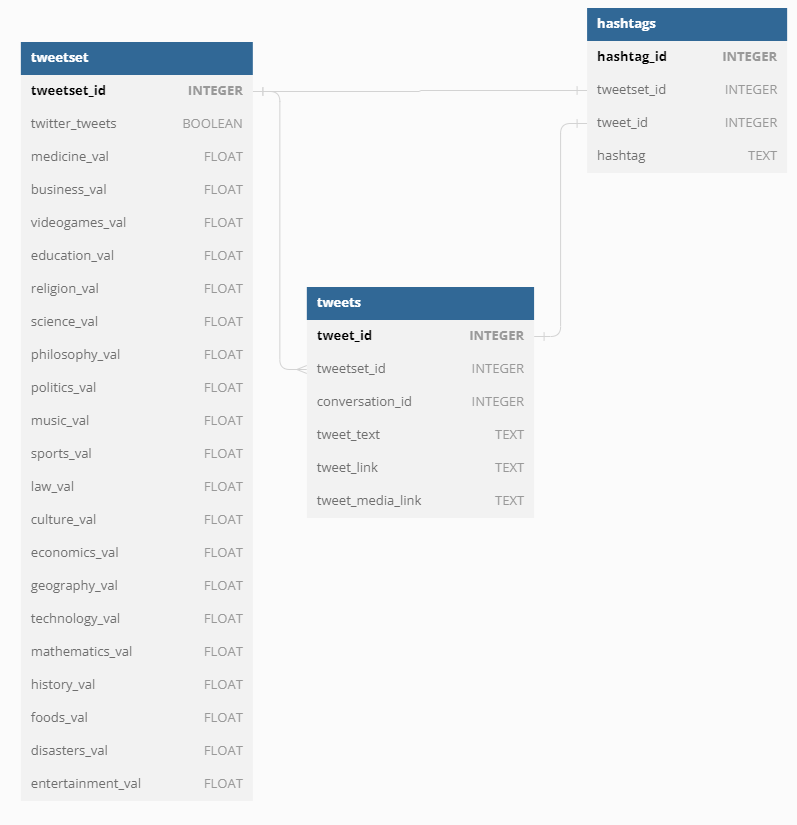
\includegraphics[width=0.8\textwidth]{images/database.png}
    \caption{Database Schema}
    \label{fig:database}
\end{figure}
The information required can be accessed using a set of queries. The implementation specifics of these queries will be discussed in Chapter \ref{ch:implementation}.